\documentclass[11 pt]{beamer}
\let\Tiny=\tiny

\usepackage{mathtools}
\usepackage{amsfonts}
\usepackage{amsmath}
\usepackage{bm}
\usepackage{graphicx}
\usepackage{pgfpages}
\usepackage[]{xcolor}
\usepackage{tikz}
\usepackage{subcaption}
\usepackage{float}
\usepackage{skull}
\usepackage[makeroom]{cancel}
\usepackage{latexsym}
\usepackage{listings}

\newcommand{\meo}[1]{\texttt{#1}} % My Eyes Only: notes just for me
\newcommand{\bigo}{\mathcal{O}}
\newcommand{\extra}[1]{{\color{purple} {#1}}}
\newcommand{\click}{$\bm{\star}$}
\newcommand{\gray}[1]{\color{gray}{#1}}

\usetheme{default}
\usecolortheme{beaver}
\usefonttheme{serif}


\beamertemplatenavigationsymbolsempty
\setbeameroption{show notes}

\setlength{\parskip}{2 ex}

\newif\ifpresstime
	\presstimefalse
	\presstimetrue

\mode<presentation>{
	\setbeameroption{hide notes}
}
\mode<handout>{
	\setbeameroption{show only notes}
	\pgfpagesuselayout{2 on 1}[letterpaper, border shrink=5mm]

}

\ifpresstime
		\renewcommand{\meo}[1]{}
		\date{April 13, 2018}
		\setbeameroption{hide notes}
	\else
		\setbeameroption{show notes}
		% \setbeameroption{show only notes}
		\date{\today}
	\fi

\usetikzlibrary{arrows, automata, shapes, decorations.pathmorphing}
\tikzset{
		initial text = {\scriptsize{\textsc{start}}},
		initial distance = 1 pt,
		every initial by arrow/.style={->},
		elliptic state/.style={draw,rounded rectangle},
		accepting/.style ={thick, double},
		wavy/.style={decorate, decoration={snake,amplitude=2 pt, segment length=5 pt, post length = 5 pt}},
		less wavy/.style={decorate, decoration={snake,amplitude=2 pt, segment length=3 pt, post length = 5 pt}}
	}


\title{Kleene's Theorem}
\author{James McFeeters}
\institute {Beloit College}
\begin{document}

\frame{
	\titlepage
}
\note[itemize]{
	\item Proof of Kleene's theorem
	\item Related to the popularity of regular expressions
	\item Start with an introduction to formal language theory, then prove Kleene's theorem, then go through examples and applications.
}

\begin{frame}
	\frametitle{Basic Definitions}
	\begin{itemize}
		\item Symbol
		\pause
		\item Alphabet ($\Sigma$)
		\pause
		\item String / word
		\begin{itemize}
			\pause
			\item The empty string ($\lambda$)
			\pause
			\item $|\lambda| = 0$
		\end{itemize}
		\pause
		\item Language
		\begin{itemize}
			\pause
			\item $\emptyset$
		\end{itemize}
	\end{itemize}
\end{frame}
\note{
	\textbf{Symbol:} The most basic unit of formal language theory --- like a letter in an alphabet.
	Can't be decomposed into anything and nothing can be combined into a symbol.

	\textbf{Alphabet:} A restricted set of symbols.
	0 and 1 for binary.
	We always assume that alphabets are nonempty and finite.

	\textbf{String:} or Word, a sequence of symbols.
	A string made entirely of symbols of one alphabet is called a string \textbf{over} that alphabet.
	We assume that strings are finite, but we don't assume that they are nonempty.
	\textbf{The Empty String:} Contains no symbols, is the string of length 0.
	Lambda is considered a string over any alphabet.
}
\note{
	\textbf{Language:} A set of strings. 
	The \textbf{empty} set is the language of NO strings over an alphabet.
	We could also just specify all the members of a language (like a dictionary).
	We're more interested in languages that are formed according to some rules so that we can describe the language without specifying all its members.
	We'll be dealing with the \textbf{regular languages}, which are formed using three set operations.
}


\begin{frame}
	\frametitle{Regular Operations}
	\begin{itemize}
		\item Union
		\item Concatenation
		\item Kleene Closure
	\end{itemize}
\end{frame}
\note{
	\textbf{Union:} probably familiar to everyone, all the strings from either language.

	Concatenation and Kleene Closure I need to define.

}


\begin{frame}
	\frametitle{Concatenation}
	\begin{columns}[T]
		\column{0.3\textwidth}
			\begin{block}{Strings}
				\begin{flalign*}
					w_1 &= ab &\\
					w_2 &= bc &\\
					w_1 w_2 &= abbc &\\
				\end{flalign*}
			\end{block}
		\column{0.5\textwidth}
		\pause
			\begin{block}{Languages}
				\begin{flalign*}
					AB &= \{ ab \mid a \in A, \, b \in B \} &\\
				\end{flalign*}
			\end{block}
	\end{columns}
	\begin{columns}[T]
		\column{0.3\textwidth}
		\pause
			\begin{flalign*}
				w^0 &= \lambda 		& \\
				w^1 &= w 			& \\
				w^2 &= ww			& \\
				w^k &= w w^{k-1} 	&
			\end{flalign*}
		\column{0.5\textwidth}
		\pause
			\begin{flalign*}
				A^0 &= \{ \lambda\} 					& \\
				A^1 &= A 							& \\
				A^2 &= AA = \{ xy \mid x, y \in A \}	& \\
				A^k &= A A^{k-1}
			\end{flalign*}
	\end{columns}
\end{frame}
\note[itemize]{
	\item Concatenation of strings is simple --- just bolt one string onto the end of the other: ``run'' and ``way'' to get runway.

	\item For languages, we use the set product. 
		Any word of the first language concatenated with any word of the second language.

	\item A bit of notation that will make the Kleene Closure easier to understand.

	\item We use superscripts to denote concatenating a word with itself, or repeating the word some number of times.
		So repeating a word zero times gets us the empty string.

	\item The same is true for languages. 
		But note that repeating a language $n$ times doesn't get us all the strings in that language repeated $n$ times, it gets us any combination of $n$ words from that language.

}

\begin{frame}
	\frametitle{Kleene Closure}
	$A^*$: the \textbf{Kleene closure} of $A$.
	\pause
	\begin{align*}
		A^* &= \bigcup_{k \geq 0} A^k \\
		&= \{ \lambda \} \cup A \cup A^2 \cdots \\
	\end{align*}
	\pause
	If $A = \{ w \}$ then $A^* = \{ \lambda, \: w, \: ww, \: www, \: \dots\}$.\\[2 ex]
	\pause
	$\Sigma^*$: all strings over $\Sigma$.
\end{frame}
\note[itemize]{
	\item The Kleene closure of a language is that language repeated any number of times.
	\item If you have a language of just one word, you get the empty string, or that word repeated any number of times.
	\item So the Kleene closure of an alphabet is all the possible strings over the alphabet.


}

\begin{frame}
	\frametitle{Regular Languages}

	The \textbf{atomic} regular languages over an alphabet $\Sigma$ are
	\pause
	\begin{itemize}
		\item $\emptyset$
		\item $\{ \lambda \}$
		\item $\{ a \}$ for any $a \in \Sigma$ 
	\end{itemize}~\\[1 em]
	\pause

	If $A$ and $B$ are regular languages, then so are
	\begin{itemize}
		\item $A \cup B$
		\item $AB$
		\item $A^*$
	\end{itemize}
\end{frame}
\note[itemize]{
	\item The \textbf{atomic} regular languages are the regular languages over any arbitrary alphabet.
	\item They are the basis for all other regular languages.
	\item[\click] The language containing no strings.
	\item[\click] The language containing just the empty string.
	\item[\click] The language containing a one-symbol string for each symbol in the alphabet.
	\item[\click] And if $A$ and $B$ are regular languages, then so are their union, concatenation, and Kleene Closure.
	\item (next slide) Two ways of representing languages.
}

\begin{frame}
	\frametitle{Regular Expressions}
	Atomic regular expressions:
	\begin{itemize}
		\item $\emptyset$ means $\emptyset$
		\item $\lambda$ means $\{ \lambda \}$;
		\item $a$ means $\{ a \}$ for any $a \in \Sigma$.
	\end{itemize}~\\[1 ex]

	If $\alpha$ means $A$ and $\beta$ means $B$, then
	\begin{itemize}
		\item $\alpha \beta$ means $AB$;
		\item $\alpha + \beta$ means $A \cup B$;
		\item $\alpha^*$ means $A^*$.
	\end{itemize}
	
\end{frame}
\note[itemize]{
	\item The first is regular expressions
	\begin{itemize}
		\item Look pretty much the same as the set notation.
		\item We drop some braces
		\item We use a plus instead of the union symbol. Read ``alpha OR beta''.
		\item Difference: two regular expressions are considered distinct, even if the languages they describe are exactly the same.
	\end{itemize}
}


\begin{frame}
	\frametitle{Finite Automata}
	\pause
	5-tuple: $M = (Q, \Sigma, s, \delta, F)$

	\begin{itemize}
		\pause
		\item [$Q$] the set of possible states. (Typically $q_1, q_2, \dots$.)
		\pause
		\item [$\Sigma$] the alphabet of input symbols.
		\pause
		\item [$s$] the initial state, $s \in Q$.
		\pause
		\item [$\delta$] the transition function:
		\pause
		\[
			\delta: (Q \times \Sigma) \to Q.
		\]
		\pause
		\item [$F$] the set of accepting states, $F \subseteq Q$.
	\end{itemize}
\end{frame}
\note{
	A \textbf{Finite automaton} is a machine with five parts.
	It has a finite number of configurations, which we call states.
	It moves between states when it receives an input symbol.
	Elevator example. (DON'T RAMBLE)
	We deal with machines that either \textbf{accept or reject} a string of inputs, based on the state of the machine after the input string.
	\begin{itemize}
		\item $Q$ is a set of states, really a set of names for states.
		These names are basically meaningless, typically they're just numbered.
		\item $\Sigma$ is the set of possible input symbols.
		\item $s$ is the state the machine starts in, before reading any input.
		\item $\delta$ tells the machine which state it should move to, given the current state and an input symbol, it outputs the next state.
		\item $F$ is all the states in which the machine is accepting the current input. Also sometimes called final states.
	\end{itemize}
}


\begin{frame}
	\frametitle{Building a Finite Automaton}
	Recognize binary numbers divisible by 3.
	\begin{center}
	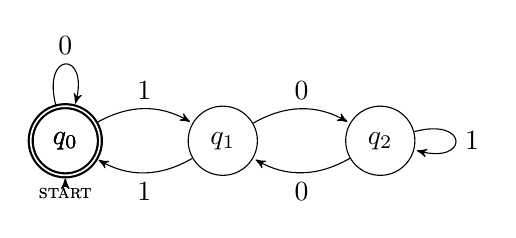
\begin{tikzpicture}[>=stealth',shorten >=1pt,auto,node distance=2cm, initial below]
		\pause % 1
		\temporal<3>
		{\node[state] (q0)                     {$q_0$};}
		{\node[state, initial] (q0)            {$q_0$};}
		{\node[state, initial, accepting] (q0) {$q_0$};}
		\node[state]                   (q1) [right of = q0] {$q_1$};
		\node[state]                   (q2) [right of = q1] {$q_2$};
		\pause % 2 Plain q0
		\pause % 3 Initial q0
		\pause % 4 Accepting q0
		\pause % 5 Show Sigma
		\path[->] (q0) edge [loop above] node {0} (q0);
		\pause % 6
		\path[->] (q0) edge [bend left]  node {1} (q1);
		\pause % 7
		\path[->] (q1) edge [bend left]  node {0} (q2);
		\pause % 8
		\path[->] (q1) edge [bend left]  node {1} (q0);
		\pause % 9
		\path[->] (q2) edge [bend left]  node {0} (q1);
		\pause % 10
		\path[->] (q2) edge [loop right] node {1} (q2);
	\end{tikzpicture}
	\end{center}
	\visible<2->{$Q = \{ q_0, q_1, q_2 \}$}\\
	\visible<3->{$\ s = q_0$}\\
	\visible<4->{$F = \{ q_0 \}$}\\
	\visible<5->{$\Sigma = \{ 0, 1 \}$}
	~\\[2 ex]
	\visible<12->{$0 \to 2 x \mod 3$}\\
	\visible<12->{$1 \to (2 x + 1) \mod 3$}
\end{frame}
\note[itemize]{
	\item Build a finite automaton to accept binary numbers divisible by 3. (reading from the most significant bit).
	\item One state per possible value mod 3
	\item We start at 0, 
	\item We accept strings divisible by 3, so $q_0$ is our only accepting state
	\item The possible input symbols are obviously 0 and 1.
	\item Now go through the transitions.
	\item $0 \to(x \mod 3) \cdot 2$

}

\begin{frame}
	\frametitle{More Fun with Automata}
	Extending the transition function:
	\pause
	\[
		\Delta : (Q \times \Sigma^*) \to Q
	\]
	\pause
	For $abc \in \Sigma^*$:
	\begin{align*}
		\Delta(q_1, abc) &= \delta \big( \Delta(q_1, ab), c \big) \\
		& = \delta \Big( \delta \big( \delta(q_1, a), b \big), c \Big) \\
	\end{align*}
	
	\pause
	\iffalse
	No transitions on $\lambda$:
	\[
		\Delta(q_i, \lambda) = q_i
	\]
	\fi
	\begin{figure}
	\centering
		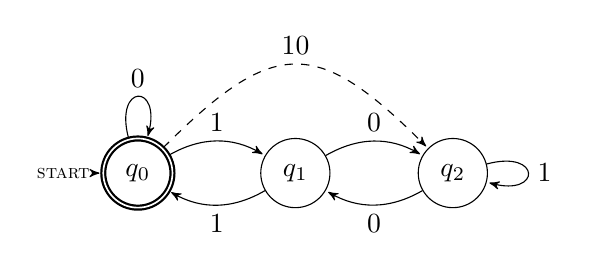
\begin{tikzpicture}[>=stealth',shorten >=1pt,auto,node distance=2cm]
			\node[initial,state,accepting] (q0)                {$q_0$};
			\node[state]                   (q1) [right of = q0] {$q_1$};
			\node[state]                   (q2) [right of = q1] {$q_2$};

			\path[->]            (q0) edge [loop above] node {0} (q0);
			\path[->]            (q0) edge [bend left]  node {1} (q1);
			\path[->]            (q1) edge [bend left]  node {0} (q2);
			\path[->]            (q1) edge [bend left]  node {1} (q0);
			\path[->]            (q2) edge [bend left]  node {0} (q1);
			\path[->]            (q2) edge [loop right] node {1} (q2);
			\pause
			\path[->] (q0) edge [loop, above, dashed, distance = 2 cm] node {10} (q2);
		\end{tikzpicture}
	\end{figure}

\end{frame}
\note[itemize]{
	\item We want to talk about the state of the machine after a string of inputs, not just after each symbol, so we want to extend the transition function
	\item So now we have a transition on any string, not just on a symbol.
	\item Define this by chaining together applications of the original transition function.
	\item We don't transition on the empty string (although it's equally valid to define automata that have lambda-transitions.)
}

\begin{frame}
	\frametitle{Finite Automata and Languages}
	The machine \textbf{accepts} $w$ if $\Delta(s, w) \in F$.\\[2 ex]
	\pause

	A machine \textbf{represents} $L(M) = \{ w \in \Sigma^* \mid \Delta(s, w) \in F \}$. \\[2 ex]
	\pause

	A language is \textbf{representable} if it can be represented by finite automaton.
\end{frame}
\note[itemize]{
	\item The machine accepts all the strings that take it from its start state to an accepting state
	\item The machine represents OR recognizes the language of all strings that take it from $s$ to an accepting state.
	\item Representable language --- can be represented by a finite automaton.
}

\begin{frame}
	\frametitle{Nondeterministic Automata}
	An automaton with multiple (or no) transitions from a state on a symbol?\\
	\pause
	Or transitions on $\lambda$?
	\pause
	\begin{center}
	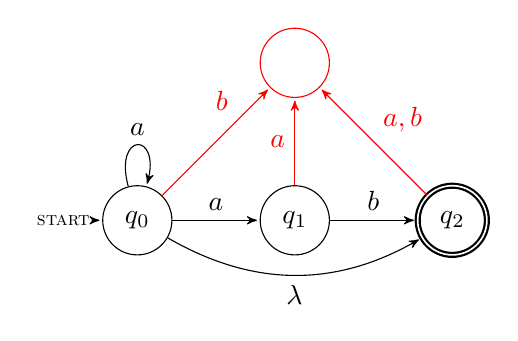
\begin{tikzpicture}[>=stealth',shorten >=1pt,auto,node distance=2cm]
		\node[state, initial]   (q0)                 {$q_0$};
		\node[state]            (q1) [right of = q0] {$q_1$};
		\node[state, accepting] (q2) [right of = q1] {$q_2$};
		\visible<5->{
			\node[state, red]   (qx) [above of = q1] {$\skull$};
		}

		\path[->] (q0) edge [loop above]        node {$a$}       (q0);
		\path[->] (q0) edge                     node {$a$}       (q1);
		\path[->] (q1) edge                     node {$b$}       (q2);
		\path[->] (q0) edge [bend right, below] node {$\lambda$} (q2);

		\visible<5->{
			\path[->] (q0) edge    [red, pos = 0.7] node {$b$}    (qx);
			\path[->] (q1) edge    [red]            node {$a$}    (qx);
			\path[->] (q2) edge    [red, swap]      node {$a, b$} (qx);
		}
	\end{tikzpicture}
	\end{center}
	\pause
	Accepts $\lambda \text{ or } ab, \, aab, \, aaab, \dots$.
\end{frame}
\note[itemize]{
	\item All the automata we've dealt with so far have exactly one transition from each state on each input, but this is not actually required.
	Automata with this restriction are DFAs.
	\item We can build automata without this restriction: they are called nondeterministic, abbreviated to NDFA.
	\item This automaton has two transitions from $q_0$ on $a$, to itself and to $q_1$. 
	\item Multiple transitions means more than one state ``active''.
	\item No transition $\implies$ dead state.
			There is no transition from $q_1$ on $a$, and no transition from $q_0$ on $b$.
	\item Talk about how it behaves.
}

\begin{frame}
	\frametitle{NDFAs are Tricky}
	We no longer have transitions to a single state.
	\[
		\delta : (Q \times \Sigma) \to \{ p \mid p \subseteq Q \}
	\]
	(to the set of all subsets of $Q$)\\[2 ex]

	\pause
	We write
	\[
		q_1 \in \delta(q_0, a) %\quad \text{ or } \quad q_1 \in \Delta(q_0, a)
	\]
	instead of 
	\[
		\delta(q_0, a) = q_1. %\quad \text{ or } \quad \Delta(q_0, a) = q_1
	\]
	~\\[2 ex]
	\pause
	An NDFA accepts $w$ if
	\[
		\Delta(s, w) \subseteq F.
	\]


\end{frame}
\note[itemize]{
	\item any subset of the states may be active at once, so we need define transitions to the power set of $Q$.
	\item Rather than say that a state IS EQUAL TO the result of a transition, we say that it is IN the result of the transition.
	\item An NDFA is accepts an input if any of its accepting states are active.
}

\begin{frame}
	\frametitle{Kleene's Theorem}
	A language representable if and only if it is regular.

	\begin{enumerate}
		\pause
		\item All regular languages are represented by an NDFA.
		\pause
		\item A language is representable by an NDFA if and only if it is representable by a DFA.
		\pause
		\item All representable languages are regular.
	\end{enumerate}
\end{frame}
\note[itemize]{
	\item A language is representable by a finite automaton if and only if it is regular.
	\item We prove this in three parts
	\item [\click] All regular languages are representable by an NDFA
	\item [\click] NDFAs and DFAs are equivalent, they represent the same family of languages.
	\item [\click] All representable languages are regular.
}


\begin{frame}
	\frametitle{The Atomic Regular Languages are Representable}
	\begin{figure}[H]
		\centering
		\visible<1->{
			\begin{subfigure}[b]{0.3 \textwidth}
				\centering
				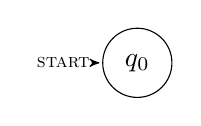
\begin{tikzpicture}[>=stealth',shorten >=1pt,auto,node distance=2cm]
					\node[initial,state] (q0)                {$q_0$};
				\end{tikzpicture}
				\caption*{Accepts $\emptyset$}
			\end{subfigure}
		}
		\visible<2->{
			\begin{subfigure}[b]{0.3 \textwidth}
				\centering
				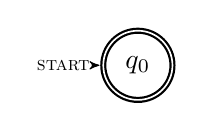
\begin{tikzpicture}[>=stealth',shorten >=1pt,auto,node distance=2cm]
					\node[initial,state, accepting] (q0)                {$q_0$};
				\end{tikzpicture}
				\caption*{Accepts $\{ \lambda \}$}
			\end{subfigure}
		}
		\visible<3->{
			\begin{subfigure}[b]{0.3 \textwidth}
				\centering
				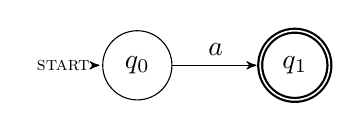
\begin{tikzpicture}[>=stealth',shorten >=1pt,auto,node distance=2cm]
					\node[initial,state]    (q0)                 {$q_0$};
					\node[state, accepting] (q1) [right of = q0] {$q_1$};
					\path[->](q0) edge  node {$a$} (q1);
				\end{tikzpicture}
				\caption*{Accepts $\{ a \}$}
			\end{subfigure}
		}
	\end{figure}
\end{frame}
\note[itemize]{
	\item We first show that all the atomic regular languages are representable by constructing NDFAs to represent them.
	\item Then we construct automata for regular combinations
	\item It's easy to construct a machine that represent the empty set --- it just has to accept no strings at all.
	\item To accept just the empty string, we have an initial state that is accepting, and define no transitions. 
	(implicit is no transition means transition to dead state.)
	\item This should make the difference between the empty set and the empty string clear.
	\item Finally, single symbol.
}

\begin{frame}
	\frametitle{Combining Representable Languages}
	\begin{figure}[H]
		\centering
			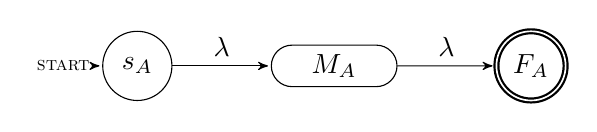
\begin{tikzpicture}[>=stealth',shorten >=1pt,auto,node distance=2.5cm, initial left]
				\node[initial,state]    (q0)                   {$s_A$};
				\node[elliptic state]   (ma)  [right of  = q0] {$\quad M_A \quad$};
				\node[state, accepting] (fa)  [right of = ma]  {$F_A$};
				\path[->](q0) edge node {$\lambda$} (ma);
				\path[->](ma) edge node {$\lambda$} (fa);
			\end{tikzpicture}
			\caption*{$L(M_A) = A$}
		\end{figure}~\\[2 em]
		\begin{figure}[H]
			\begin{tikzpicture}[>=stealth',shorten >=1pt,auto,node distance=2.5cm, initial left]
				\node[initial,state]    (q0)                   {$s_B$};
				\node[elliptic state]   (mb)  [right of  = q0] {$\quad M_B \quad$};
				\node[state, accepting] (fb)  [right of = ma]  {$F_B$};
				\path[->](q0) edge node {$\lambda$} (mb);
				\path[->](mb) edge node {$\lambda$} (fb);
			\end{tikzpicture}
			\caption*{$L(M_B) = B$}
		\end{figure}
\end{frame}
\note{
	If languages are representable we have machines that represent them.
	So we can combine these machines to represent combinations of the languages.\\[2 ex]

	Introduce my rough diagrams.
	Mention that the sets of states are not shown with perfect accuracy.

	\begin{itemize}
		\item $s$ is the start state
		\item $F$ is all the accepting states
		\item $M_A$ represents any state of the machine
		\item First arrow represents transitions from the initial state to any state of the automaton
		\item And the second arrow represents transitions from any state to any accepting state.
	\end{itemize}

}

\begin{frame}
	\frametitle{Union of Representable Languages}
	\begin{figure}[H]
		\centering
		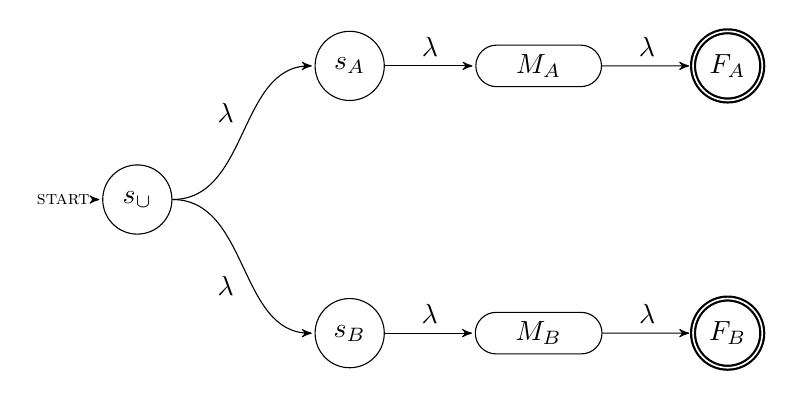
\begin{tikzpicture}[>=stealth',shorten >=1pt,auto,node distance=2.4cm, initial left]
			\visible<2->{
				\node[initial,state]    (sab)                             {$s_\cup$};
			}

			\visible<1->{
				\node[state]            (sa)  [above right of = sab, xshift = 1 cm]      {$s_A$};
				\node[elliptic state]   (ma)  [right of = sa]                            {$\quad M_A \quad$};
				\node[state,accepting]  (fa)  [right of = ma]                            {$F_A$};
				\path[->](sa) edge node {$\lambda$} (ma);
				\path[->](ma) edge node {$\lambda$} (fa);

				\node[state]            (sb)  [below right of = sab, xshift = 1 cm]      {$s_B$};
				\node[elliptic state]   (mb)  [right of = sb]                            {$\quad M_B \quad$};
				\node[state, accepting] (fb)  [right of = mb]                            {$F_B$};
				\path[->](sb) edge node {$\lambda$} (mb);
				\path[->](mb) edge node {$\lambda$} (fb);
			}
			\visible<3->{
				\path[->](sab) edge [out=0, in=180]       node {$\lambda$} (sa);
				\path[->](sab) edge [out=0, in=180, swap] node {$\lambda$} (sb);
			}
		\end{tikzpicture}
	\end{figure}
\end{frame}
\note[itemize]{
	\item Need a machine to accept strings from either language.
	\item Connect $M_A$ and $M_B$ in parallel.
	\item keep all the states of $M_A$ and $M_B$
	\item Keep all the accepting states of $M_A$ and $M_B$.
	\item[\click] Add a new initial state which we'll link into both machines
	\item[\click] If either language contains the empty string, $s_\cup$ is accepting.
	\item[\click] Add transitions from $s_\cup$ to mimic those from $s_A$ and $s_B$.

}

\begin{frame}
	\frametitle{Concatenation of Representable languages}
	\begin{figure}[H]
		\centering
			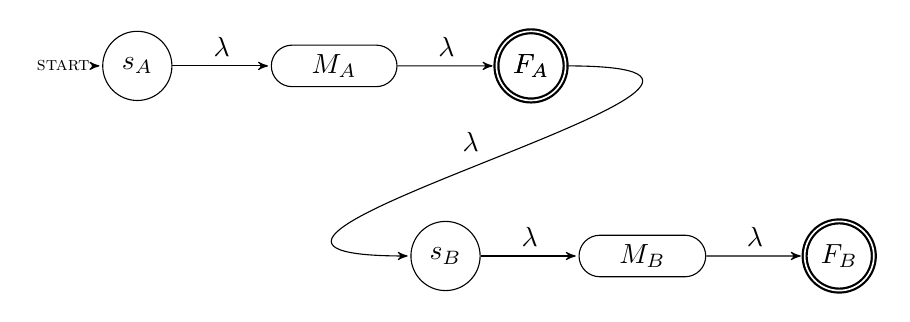
\begin{tikzpicture}[>=stealth',shorten >=1pt,auto,node distance=2.5cm, initial left]
				\node[initial,state]    (sab)                   {$s_A$};
				\node[elliptic state]   (ma)  [right of = sab]  {$\quad M_A \quad$};
				\alt<2->
					{\node[state]            (fa)  [right of = ma]   {$F_A$};}
					{\node[state, accepting] (fa)  [right of = ma]   {$F_A$};}
				\path[->](sab) edge node {$\lambda$} (ma);
				\path[->](ma)  edge node {$\lambda$} (fa);

					\node[state]            (sb)  [below right of = ma, node distance = 2cm, yshift = -1 cm]  {$s_B$};
					\node[elliptic state]   (mb)  [right of = sb]                                             {$\quad M_B \quad$};
					\node[state, accepting] (fb)  [right of = mb]                                             {$F_B$};
					\path[->](sb) edge node {$\lambda$} (mb);
					\path[->](mb) edge node {$\lambda$} (fb);

				\visible<3->{
					\path[->](fa) edge  [out=0, in=180, distance=4cm, swap] node {$\lambda$}          (sb);
				}
			\end{tikzpicture}
	\end{figure}
\end{frame}
\note[itemize]{
	\item Needs to accept strings of $A$ concatenated with strings of $B$.
	\item Connect the two machines in series
	\item Keep all the states of both machines
	\item The initial state of the new machine is the start state of $M_A$.
	\item The accepting states of $M_A$ are no longer accepting --- a string of $A$ needs to be followed by a string of $B$.
	\item The accepting states are the accepting states of $M_B$. 
	\item[\click] Add transitions to $s_B$ shadowing those into $F_A$
	\item[\click] If lambda is in $B$, then $s_B$ is an accepting state.
	\item[\click] $s_A$ is accepting if lambda is in both $A$ and $B$.
	\item[\click] If lambda in $A$, add transitions from $s_A$ that mimic those from $s_B$.
}

\begin{frame}
	\frametitle{Kleene Closure of a Representable Language}
	\begin{figure}[H]
		\centering
			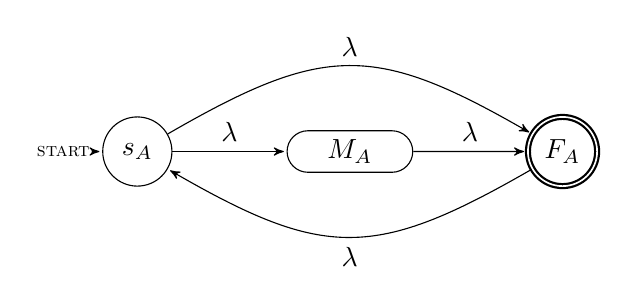
\begin{tikzpicture}[>=stealth',shorten >=1pt,auto,node distance=2.7cm, initial left]
				\node[state, initial]            (sa)        {$s_A$};

				\visible<1->{
					\node[elliptic state]   (ma)  [right of = sa] {$\quad M_A \quad$};
					\node[state,accepting]  (fa)  [right of = ma] {$F_A$};
					\path[->](sa) edge node {$\lambda$} (ma);
					\path[->](ma) edge node {$\lambda$} (fa);
				}
				\visible<2->{
					\path[->](sa) edge [bend left, above, distance = 2.3 cm] node {$\lambda$} (fa);
				}
				\visible<3->{
					\path[->](fa) edge [bend left, below, distance = 2.3 cm] node {$\lambda$} (sa);
				}
			\end{tikzpicture}
	\end{figure}
\end{frame}
\note[itemize]{
	\item add a new start state, accepting to accept $\lambda$.
	\item add transitions from $s_{A*}$ shadowing the transitions from $s_A$.
	\item Link $M_A$ to itself to form a circle.
	\item add transitions from every state in $F_A$ that mimic those from $s_A$.
	\item Now we have all the operations and all the atomics, so we can represent all the regular languages.
}

\begin{frame}
	\frametitle{What's Next?}
	A language representable if and only if it is regular.

	\begin{enumerate}
		\item[$\checkmark $1.] All regular languages are represented by an NDFA.
		\item[2.] A language is representable by an NDFA if and only if it is representable by a DFA.
		\item[3.] All representable languages are regular.
	\end{enumerate}
\end{frame}

\begin{frame}
	\frametitle{NDFAs and DFAs are Equivalent}
	\textit{A language is representable by an NDFA if and only if it is representable by a DFA.}\\[1 em]
	\pause
	All DFAs are NDFAs: nothing to prove in that direction.\\[1 em]

	\pause
	For an NDFA $M = (Q, \Sigma, s, \delta, F)$ construct a DFA $M'$ such that
	\[
		L(M') = L(M).
	\]
\end{frame}
\note[itemize]{
	\item We need to show that any language represented by an NDFA can be represented by a DFA, and vice-versa.
	\item All DFAs are actually NDFAs already, so we don't have to worry about the vice-versa part.
	\item For any NDFA, we need to construct a DFA that accepts the same language.
	\item I'm just going to skim over the construction we use.
}

\begin{frame}
	\frametitle{Power Set Construction}
	\begin{itemize}
		\setlength\itemsep{2 ex}
		\pause
		\item[] $Q' = \{ p \mid p \subseteq Q \}$\\[1 ex]
		$\{ q_1, q_2, \dots, q_n \} \subseteq Q \quad \implies \quad \{ q_1, q_2, \dots, q_n \} \in Q'$.
		\pause
		\item[] $s' = \{ s \}$
		\pause
		\item[] $F' = \{ p \in Q' \mid p \cap F \neq \emptyset \}$
	\end{itemize}
	~\\[2 em]
	\pause
	We have 
	\begin{align*}
		M' = (Q', \Sigma, \{ s \}, \delta', F')
	\end{align*}
	
\end{frame}
\note[itemize]{
	\item Any subset of the states of $M$ may be active at any given time, so we need one state in $M'$ to represent each subset of $Q$.
	\item[\click] Thus the set of states for our DFA is the power set of the states of our NDFA.
	\item[\click] The initial state of $M'$ is the subset containing just the initial state of $M$.
	\item[\click] The accepting states of $M'$ are all the subsets that contain an accepting state of $M$.
	\item[\click] Everything except the transition function is defined

}

\begin{frame}
	\frametitle{Power Set Construction}
	For $a \in \Sigma$ define,
		\begin{align*}
			\delta'(\{ q_1, q_2, \dots, q_n \}, a) &= \delta(q_1, a) \cup \delta(q_2, a) \cup \cdots \cup \delta(q_n, a) \\
			&= \bigcup_{i = 1}^n \delta(q_i, a)
		\end{align*}

	\pause
	This works because
	\[
		\Delta'(\{ s \}, w) = \Delta(s, w) \quad \text{for all } w \in \Sigma^*
	\]
	which implies
	\[
		\Delta'(\{ s \}, w) \in F' \iff \Delta(s, w) \subseteq F.
	\]
\end{frame}
\note[itemize]{
	\item[\click] The transitions in $M'$ are defined as a union of transitions in $M$.
	\item[\click] This works because the active state in the DFA always corresponds exactly to the set of active states in the original NDFA
	\item Thus the set of inputs that lead to an accepting state correspond exactly. 
}

\begin{frame}
	\frametitle{Power Set Construction Example}
	\begin{columns}
	\column{0.4 \textwidth}
		\begin{figure}[H]
			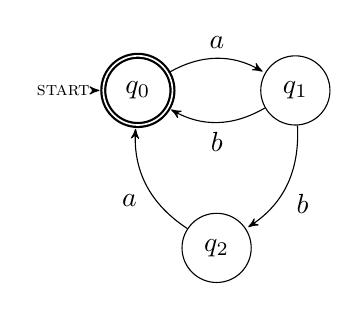
\begin{tikzpicture}[>=stealth',shorten >=1pt,auto,node distance=2cm]
				\node[state, initial, accepting] (q0)                       {$q_0$};
				\node[state]                     (q1) [right of = q0]       {$q_1$};
				\node[state]                     (q2) [below of = q0, xshift = 1 cm] {$q_2$};
				
				\path[->] (q0) edge [bend left] node {$a$}       (q1);
				\path[->] (q1) edge [bend left] node {$b$}       (q0);
				\path[->] (q1) edge [bend left] node {$b$}       (q2);
				\path[->] (q2) edge [bend left] node {$a$}       (q0);
			\end{tikzpicture}
		\end{figure}
	\column{0.6 \textwidth}
		This is $M$.

		$M$ accepts $(a(b + ba))^* = (ab+aba)^*$.

		We want to construct a DFA $M'$.

	\end{columns}
	\alt<-2>
	{$Q' = \big\{ \emptyset, \{ q_0 \}, \{ q_1 \}, \{ q_2 \}, \{ q_0, q_1 \}, \{ q_0, q_2 \}, \{ q_1, q_2 \}, \{ q_0, q_1, q_2 \} \big\}$}
	{$Q' = \big\{ \emptyset, \{ q_0 \}, \{ q_1 \}, \cancel{\{ q_2 \}}, \{ q_0, q_1 \}, \{ q_0, q_2 \}, \cancel{\{ q_1, q_2 \}}, \cancel{\{ q_0, q_1, q_2 \}} \big\}$}
	\pause
	\pause

	\pause
	$s' = \{ q_0 \}$

	\pause
	$F' = \{ \{ q_0 \}, \{ q_0, q_1 \}, \{ q_0, q_2 \} \}$


\end{frame}

\begin{frame}
	\frametitle{What's Next?}
	A language representable if and only if it is regular.

	\begin{enumerate}
		\item[$\checkmark $1.] All regular languages are represented by an NDFA.
		\item[$\checkmark $2.] A language is representable by an NDFA if and only if it is representable by a DFA.
		\item[3.] All representable languages are regular.
	\end{enumerate}
\end{frame}

\begin{frame}
	\frametitle{All Representable Languages are Regular}

	\textit{We can construct a regular expression to describe the language accepted by any DFA.}\\[1 em]
	\pause

	Let $M$ be a DFA with states $Q = \{ q_1, q_2, \dots, q_n \}$
	\pause

	$1 \leq i, j \leq n$.
	\pause

	Look at paths $q_i \leadsto q_j$. 
	\pause

	$0 \leq k \leq n$.

	Look at paths $q_i \leadsto q_j$ that do not pass through any state numbered higher than $k$.
	\pause

	$R_k(i, j)$ describes the words that label these paths.



\end{frame}
\begin{frame}
	\frametitle{Regular Expressions for Direct Transitions}
	Start with $k = 0$ \hspace{1 ex} (No intermediate states allowed.)
	\pause

	$R_0(i, j)$ describes the \textbf{direct} transitions from $q_i$ to $q_j$.
	\pause

	\begin{align*}
		R_0(i, j) &= 
		\begin{cases}
			\{ a \in \Sigma \mid \delta(q_i, a) = q_j \} 			& \text{ if } i \neq j \\
			\{ a \in \Sigma \mid \delta(q_i, a) = q_j \} + \lambda 	& \text{ if } i = j
		 \end{cases}\\[2 ex]
		\uncover<4->{
			&=
			\begin{cases}
				\emptyset \\
				a_1 + a_2 + \cdots \\
				\lambda \\
				\lambda + a_1 + a_2 + \cdots
			\end{cases}
			\ (a_1, a_2, \dots \in \Sigma)
		}
	\end{align*}
	\pause % I've forgotten the Act of Contrition
	\pause
	These are all regular!
\end{frame}


\begin{frame}
	\frametitle{Regular Expressions for Indirect Transitions}

	\begin{align*}
		R_1(i, j) &= R_0(i, j) + \big(R_0(i, 1) \ (R_0(1, 1))^* \ R_0(1, j) \big) \\[1 ex]
		\uncover<2->{
			R_{k+1}(i, j) &= R_k(i, j) + \big( R_k(i, k\!+\!1) \ \big(R_k(k\!+\!1, k\!+\!1)\big)^* \ R_k(k\!+\!1, j) \big)
		}
	\end{align*}
	\pause % uncover line 2.

	\pause
	\begin{figure}[H]
		\centering
		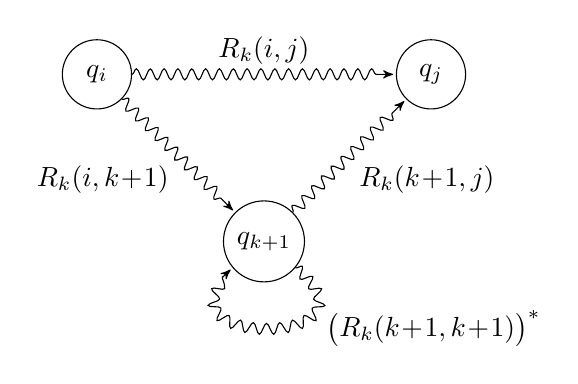
\begin{tikzpicture}[>=stealth',shorten >=1pt,auto,node distance=3cm]
			\visible<4->{
			\node[state]            (qk)                       {$q_{k+1}$};}
			\node[state]            (qi) [above left of = qk]  {$q_i$};
			\node[state]            (qj) [above right of = qk] {$q_j$};
			
			\path[->] (qi) edge   [wavy]                                                            node {$R_k(i, j)$}     (qj);

			\visible<5->
			{\path[->] (qi) edge   [wavy, swap]                                                      node {$R_k(i, k\!+\!1)$}     (qk);}

			\visible<6->
			{\path[->] (qk) edge   [wavy, loop, out = 320, in = 220, looseness = 5, pos = 0.17]      node {$\big(R_k(k\!+\!1, k\!+\!1)\big)^*$} (qk);}

			\visible<7->
			{\path[->] (qk) edge   [wavy, swap]                                                      node {$R_k(k\!+\!1, j)$}     (qj);}
		\end{tikzpicture}
		\caption*{\gray{Adapted from Harrison \cite[pg.~59]{lemmings}}}
	\end{figure}
\end{frame}


\begin{frame}
	\frametitle{Example}
	\begin{figure}[H]
		\centering
		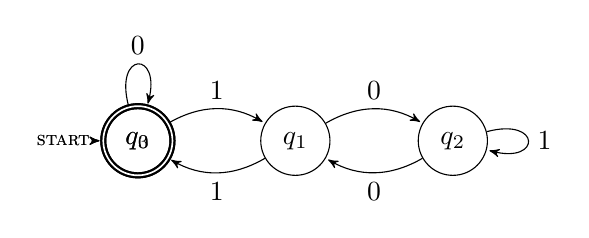
\begin{tikzpicture}[>=stealth',shorten >= 1 pt, auto, node distance = 2 cm]
			\alt<-2>
			{\node[initial,state,accepting] (q0)                 {$q_0$};}
			{\node[initial,state,accepting] (q0)                 {$q_3$};}
			\node[state]                    (q1) [right of = q0] {$q_1$};
			\node[state]                    (q2) [right of = q1] {$q_2$};

			\path[->](q0) edge [loop above] node {0} (q0);
			\path[->](q0) edge [bend left]  node {1} (q1);
			\path[->](q1) edge [bend left]  node {0} (q2);
			\path[->](q1) edge [bend left]  node {1} (q0);
			\path[->](q2) edge [bend left]  node {0} (q1);
			\path[->](q2) edge [loop right] node {1} (q2);
		\end{tikzpicture}
	\end{figure}
	\pause % 2 show text
	\visible<2->
	{We need to number the states starting at 1.}
	\pause % 3 change machine
	\pause % 4

	\begin{block}{What Languages does this Accept?}
		\vspace{- 6 ex}
		\begin{align*}
			\uncover<5->{
			R_0(3, 3) &= \lambda + 0 \\
			}
			\uncover<6->{
			R_1(3, 3) &= \lambda+0 \bm{+11} \\
			}
			\uncover<7->{
			R_2(3, 3) &= (\lambda+0+11)\bm{ + 10(1+00)^*01} \\
			}
			\uncover<8->{
			R_3(3, 3) &= \pmb{\big(}0+11+(10 \, (1+00)^* \, 01)\pmb{\big)^*}
			}
		\end{align*}
	\end{block}
	\pause % 5
	\pause % 6
	\pause % 7
	\pause % 8
\end{frame}




\begin{frame}
	\frametitle{What's Next}
	A language representable if and only if it is regular.

	\begin{enumerate}
		\item[$\checkmark $1.] All regular languages are represented by an NDFA.
		\item[$\checkmark $2.] A language is representable by an NDFA if and only if it is representable by a DFA.
		\item[$\checkmark $3.] All representable languages are regular.
	\end{enumerate}
	So we have proven Kleene's theorem.
\end{frame}


\begin{frame}
	\frametitle{Applications}
	\begin{itemize}
		\pause
		\item We can convert a regular language (or expression) into an NDFA.
		\pause
		\item We can convert an NDFA into a DFA
		\pause
		\item We can minimize a DFA
		\pause
		\item We can represent a DFA as a matrix
	\end{itemize}
	\pause
	\begin{columns}
	\column{0.5 \textwidth}
		\begin{figure}[H]
			\centering
			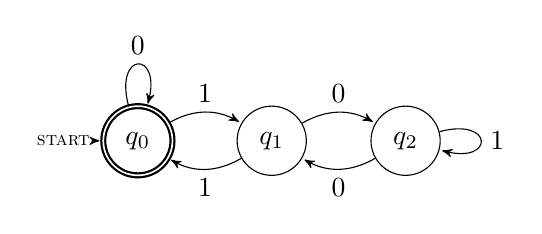
\begin{tikzpicture}[>=stealth',shorten >=1pt,auto,node distance=1.7cm]
				\node[initial,state,accepting] (q0)                {$q_0$};
				\node[state]                   (q1) [right of = q0] {$q_1$};
				\node[state]                   (q2) [right of = q1] {$q_2$};

				\path[->](q0) edge [loop above] node {0} (q0);
				\path[->](q0) edge [bend left]  node {1} (q1);
				\path[->](q1) edge [bend left]  node {0} (q2);
				\path[->](q1) edge [bend left]  node {1} (q0);
				\path[->](q2) edge [bend left]  node {0} (q1);
				\path[->](q2) edge [loop right] node {1} (q2);
			\end{tikzpicture}
		\end{figure}
	\pause
	\column{0.5 \textwidth}
		\begin{figure}[H]
			\centering
			\begin{tabular}{c c c}
								& $\mathbf{0}$ 	& $\mathbf{1}$ \\
				$\mathbf{q_0}$	& $q_0$			& $q_1$ \\
				$\mathbf{q_1}$	& $q_2$			& $q_0$ \\
				$\mathbf{q_2}$	& $q_1$			& $q_2$ \\
			\end{tabular}
		\end{figure}
	\end{columns}
	\pause
	Looking up a value in an array is $\bigo(1)$.\\
	\pause
	Looking up $N$ values in an array is $\bigo(N)$.
\end{frame}

\begin{frame}[fragile]
	\frametitle{Grep (Everyone's Favorite Unix Utility!)}
	\begin{center}
		{\small
		\begin{tabular}{|r l|}
			\hline
			\textbf{Expression} 	& \textbf{Meaning} \\
			\hline
			$\mathtt{.}$ 					& Any character \\
			$\mathtt{a}$ 					& The letter $\mathtt{a}$ \\
			$\mathtt{a?}$ 					& $\mathtt{a}$ once or zero times \\
			$\mathtt{a*}$ 					& $\mathtt{a}$ zero or more times \\
			$\mathtt{a+}$ 					& $\mathtt{a}$ one or more times \\
			$\mathtt{a \{ n, m \}}$ 		& $\mathtt{a}$ between $\mathtt{n}$ and $\mathtt{m}$ times \\
			$\mathtt{[\char`^{} abc]}$ 		& any character except $\mathtt{a}$, $\mathtt{b}$, or $\mathtt{c}$ \\
			$\mathtt{(a | b)}$ 				& either $\mathtt{a}$ or $\mathtt{b}$ \\
			\hline
		\end{tabular}
		}
	\end{center}
	\begin{block}{Examples}
	\vspace{-3 ex}
		\begin{itemize}
			\item[] \verb!a (ND)?FA!
			\item[] \verb!^\d{2}:\d{2}:\d{2}\d{1,2}\/\d{1,2}\/\d{1,2}$! 
		\end{itemize}
	\end{block}
\end{frame}

\begin{frame}[shrink]
	\frametitle{References}
	\bibliographystyle{amsplain}
	\nocite{*}
	\bibliography{../paper/references.bib}
\end{frame}


\begin{frame}[fragile]
	\frametitle{Questions?}
	\begin{figure}[H]
		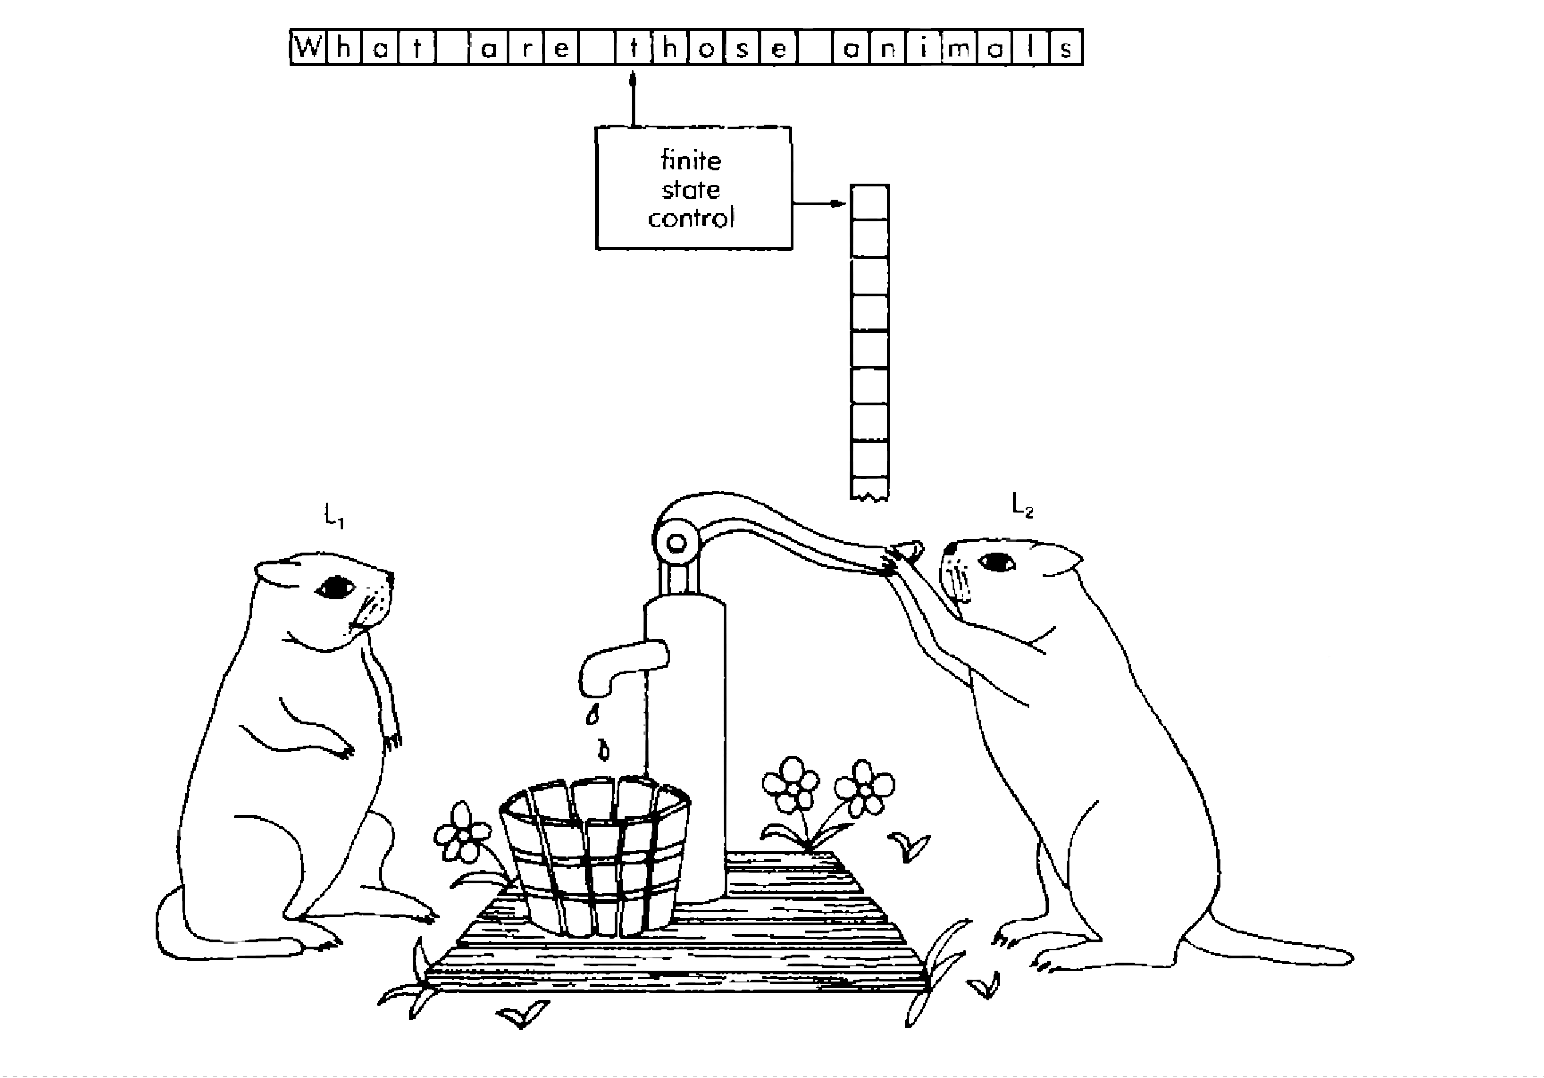
\includegraphics[width = \textwidth]{../images/pumping_lemmings.png}
	\end{figure}
\end{frame}

\begin{frame}
	\frametitle{Power Set with $\lambda$--closure}

	\centering
	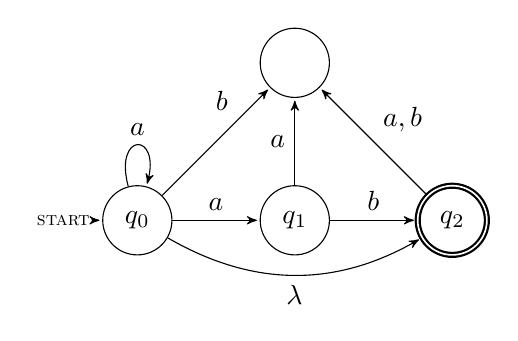
\begin{tikzpicture}[>=stealth',shorten >=1pt,auto,node distance=2cm]
		\node[state, initial]   (q0)                 {$q_0$};
		\node[state]            (q1) [right of = q0] {$q_1$};
		\node[state, accepting] (q2) [right of = q1] {$q_2$};
		\node[state]            (qx) [above of = q1] {$\skull$};
		
		\path[->] (q0) edge [loop above]        node {$a$}       (q0);
		\path[->] (q0) edge                     node {$a$}       (q1);
		\path[->] (q1) edge                     node {$b$}       (q2);
		\path[->] (q0) edge [bend right, below] node {$\lambda$} (q2);

		\path[->] (q0) edge [pos = 0.7] node {$b$}    (qx);
		\path[->] (q1) edge             node {$a$}    (qx);
		\path[->] (q2) edge [swap]      node {$a, b$} (qx);
	\end{tikzpicture}

	\begin{tikzpicture}[>=stealth',shorten >=1pt,auto,node distance=2cm]
		\node[elliptic state, initial, accepting] (q02)                  {$\{ q_0, q_2 \}$};
		\node[elliptic state]                     (q01) [right of = q02] {$\{ q_0, q_1 \}$};
		\node[state, accepting]                   (q2)  [right of = q01] {$\{q_2\}$};
		\node[state]                              (qx)  [below of = q1]  {$\emptyset$};
		
		\path[->] (q02) edge              node {$a$} (q01);
		\path[->] (q01) edge [loop above] node {$a$} (q01);
		\path[->] (q01) edge              node {$b$} (q2);

		\path[->] (q02) edge [pos = 0.7, swap]   node {$b$}    (qx);
		\path[->] (q2) edge                      node {$a, b$} (qx);
		\path[->] (qx) edge  [loop below, right] node {$a, b$} (qx);
	\end{tikzpicture}
\end{frame}

\begin{frame}
	\frametitle{A picture that is too big!}
	\centering
	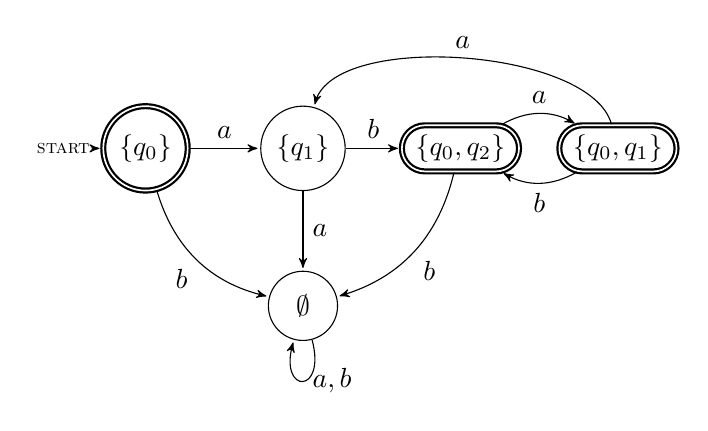
\begin{tikzpicture}[>=stealth',shorten >=1pt,auto,node distance=2cm]
		\node[state, initial, accepting] (q0)                         {$\{q_0\}$};
		\node[state]                     (q1)  [right of = q0]        {$\{q_1\}$};
		\node[elliptic state, accepting] (q02) [right of = q1]        {$\{ q_0, q_2 \}$};
		\node[elliptic state, accepting] (q01) [right of = q02]       {$\{ q_0, q_1 \}$};
		\node[state]                     (qx)  [below of = q1]        {$\emptyset$};

		\path[->] (q0)  edge                                      node {$a$} (q1);
		\path[->] (q1)  edge                                      node {$b$} (q02);
		\path[->] (q02) edge [bend left]                          node {$a$} (q01);
		\path[->] (q01) edge [bend left]                          node {$b$} (q02);
		\path[->] (q01) edge [loop above, above, distance = 1 cm] node {$a$} (q1);

		\path[->] (q0)  edge [bend right, swap]                   node {$b$}    (qx);
		\path[->] (q1)  edge                                      node {$a$}    (qx);
		\path[->] (q02) edge [bend left]                          node {$b$}    (qx);
		\path[->] (qx)  edge [loop below, right]                  node {$a, b$} (qx);

	\end{tikzpicture}
\end{frame}


\begin{frame}
	\frametitle{Matrices for Example}
	\centering

	\begin{tabular}{|r | c c c|}
		\hline
		$\bm{k=0}$	&$j = 1$ 		& $2$ 				& $3$ 			\\
		\hline
		$i = 1$ 	&$\lambda$ 		& $0$				& $1$ 				\\
		$2$ 		&$0$ 			& $\lambda + 1$ 	& $\emptyset$		\\
		$3$ 		&$1$ 			& $\emptyset$ 		& $\lambda + 0$ 	\\
		\hline
	\end{tabular}

	\begin{tabular}{|r | c c c|}
		\hline
		$\bm{k=1}$		&$j = 1$ 		& $2$ 				& $3$ 			\\
		\hline
		$i = 1$ 		& $\lambda$ 		& $0$						& $1$ 					\\
		$2$ 			& $0$ 			& $\lambda+1+\bm{00}$ 		& $\bm{01}$				\\
		$3$ 			& $1$ 			& $\bm{10}$ 				& $\lambda+0+\bm{11}$ 	\\
		\hline
	\end{tabular}

	\resizebox*{\textwidth}{!}{
	\begin{tabular}{|r| c c c|}
		\hline
		$\bm{k=2}$	& $j = 1$ 						& $2$ 						& $3$ 									\\
		\hline
		$i = 1$ 	& $\lambda + \bm{0(1+00)^*0}$ 	& $0+\bm{0(1+00)^*}$		& $1+\bm{0(1+00)^*01}$					\\[1.5 ex]
		$2$ 		& $0+\bm{(1+00)^*0}$ 			& $\bm{(}1+00\bm{)^{*}}$ 	& $\bm{(1+00)^*}01$						\\[1.5 ex]
		$3$ 		& $1+\bm{(10(1+00)^*0)}$ 		& $10\bm{(1+00)^*}$ 		& $(\lambda+0+11)+\bm{10(1+00)^*01}$ 	\\
		\hline
	\end{tabular}}
\end{frame}

\end{document}
